\documentclass[journal,12pt,twocolumn]{article}
\usepackage{graphicx}
\usepackage[none]{hyphenat}
\usepackage[margin=0.5in]{geometry}
\usepackage[cmex10]{amsmath}
\usepackage{array}
\usepackage{booktabs}
\usepackage{gensymb}
\usepackage{textcomp}
\title{\textbf{Circle Assignment}}
\author{Manideep Parusha - FWC22004}
\date{\today}

\providecommand{\norm}[1]{\left\lVert#1\right\rVert}
\providecommand{\abs}[1]{\left\vert#1\right\vert}
\let\vec\mathbf
\newcommand{\myvec}[1]{\ensuremath{\begin{pmatrix}#1\end{pmatrix}}}
\newcommand{\mydet}[1]{\ensuremath{\begin{vmatrix}#1\end{vmatrix}}}
\providecommand{\brak}[1]{\ensuremath{\left(#1\right)}}

\begin{document}

\maketitle
\section*{Problem}
\paragraph{Show that the tangents of circle drawn at the ends of diameter are parallel.}

\section*{Solution}

\begin{figure}[h]
\centering
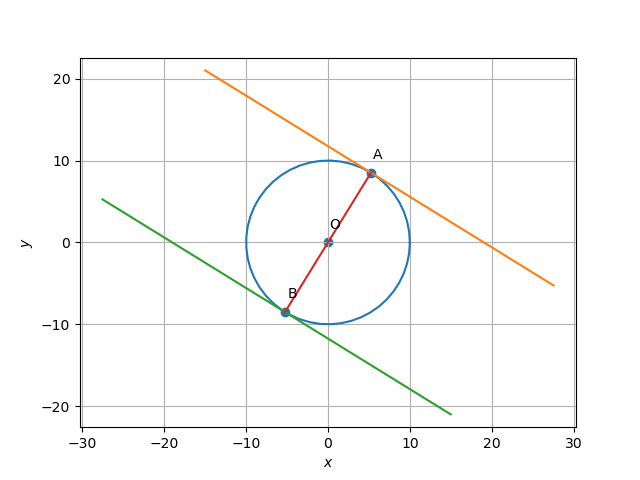
\includegraphics[width=\columnwidth]{figs/plot_cir.png}
\caption{Circle with tangents at ends of it's diameter}
\label{fig:cir_py}
\end{figure}

\subsection*{Construction}
Input taken for the construction of the Circle and the tangents is 'r' radius of the circle.

\begin{table}[h]
	\centering
\setlength\extrarowheight{2pt}
	\begin{tabular}{|c|c|c|}
		\hline
		\textbf{Symbol} & \textbf{Value} & \textbf{Description} \\
		\hline
		r & 10 & circle radius\\
		\hline
		O & $-\vec{u}$ & Center\\
		\hline
		A & \myvec{a_1\\a_2} & point A\\
		\hline
		B & \myvec{b_1\\b_2} & point B\\
		\hline
	\end{tabular}
\end{table}

Let us assume a circle with radius 'r' and center at origin.\\
\begin{align}
	\boldsymbol{x}^{T}\boldsymbol{Vx} + 2\boldsymbol{u}^{T}\vec{x} + f = 0
\end{align}
but, for a Circle 
\begin{align}
	\boldsymbol{V} = \myvec{ 1 & 0 \\0 & 1}
\end{align}
and the center of the circle is,
\begin{align}
	-\vec{u} = \myvec{u_1 \\ u_2}
	\label{center}
\end{align}
Let us assume a point $\vec{A}$ on the circle and a point $\vec{B}$ such that the points form the diameter of the circle.
%To prove that tangets at the ends of a diameter are parallel, we need to find the slope of tangents at the given points.\\
%\begin{align}
%	\vec{A} = \myvec{a_1 \\ a_2}
%\end{align}
Center of the circle bisect the diameter in equal parts. Then,
\begin{eqnarray}
	\frac{\vec{A} + \vec{B}}{2} = -\vec{u} \\
	\implies \vec{A}+\vec{B} = -2\vec{u}
	\label{ab}
\end{eqnarray}

Here, $\vec{A}$ and $\vec{B}$ are the ends of the diameter and the contact points for the tangents.
We know that, for a circle, any line passing through it's center is a normal to the circle at the point of contact.\\
Tangent intersect the circle at only one point on it's circumference.
So, the line intersecting the circle at one point $\vec{q}$ is 
\begin{align}
	\boldsymbol{m}^{T}(\boldsymbol{Vq} + \boldsymbol{u}) = 0
\end{align}
where $\boldsymbol{m}$ is the directional vector of line at the point of contact.\\
equation for a tangent at point $\vec{A}$ is
\begin{align}
	\boldsymbol{m_1}^{T}(\boldsymbol{A} + \boldsymbol{u}) = 0
	\label{eqn:t1}
\end{align}
Similarly, Euqation of the tangent at $\boldsymbol{B}$ is given by,
\begin{align}
	\boldsymbol{m_2}^{T}(\boldsymbol{B} + \boldsymbol{u}) = 0
	\label{eqn:t2}
\end{align}
where $\vec{m_1}$\&$\vec{m_2}$ are the direction vectors of the tangents.\\
%where $\boldsymbol{n}$ is the normal vector at the point of contact.\\
Then, the normal vectors at the point of contact of tangets are
\begin{equation}
	\vec{A}+\vec{u} = k_1\vec{n_1}
	\label{n1}
\end{equation}
\begin{equation}
	\vec{B}+\vec{u} = k_2\vec{n_2}
	\label{n2}
\end{equation}
by adding the above equations \eqref{n1}\&\eqref{n2}, 
\begin{align}
	\vec{A}+\vec{B} + 2\vec{u} = k_1\vec{n_1}+k_2\vec{n_2}
	\label{addeq}
\end{align}
from \eqref{ab}, \eqref{addeq} can be modified as 
 \begin{align}
	 k_1\vec{n_1}+k_2\vec{n_2} = 0 \\
	k_1\vec{n_1} = -k_2\vec{n_2}
 \end{align}
The crossproduct of the normal vectors is zero.
\begin{align}
	\vec{n_1} \times \vec{n_2} = 0
\end{align}

Here, the mormal vectors are parallel $n_1$ \& $n_2$. So the tangents are parallel to each other.\\
Hence, we have proved that the tangents at the ends of the diameter of a circle are parallel.
\end{document}
